\documentclass[12pt,a4paper]{article}
\usepackage[utf8]{inputenc}
\usepackage[T1]{fontenc}
\usepackage[brazil]{babel}
\usepackage[margin=2cm]{geometry}
\usepackage{graphicx,booktabs,float}
\usepackage[hidelinks]{hyperref}
% Gerado dos CSVs validados. Não editar números manualmente.
\newcommand{\TotalIES}{70}
\newcommand{\TotalCursos}{79}
\newcommand{\TotalInscritos}{1418}
\newcommand{\TotalPresentes}{1209}
\newcommand{\TotalNotas}{1203}
\newcommand{\TotalSuprimidos}{6}
\newcommand{\TotalAusentes}{208}
\newcommand{\TotalOutros}{1}
\newcommand{\CursosComNotas}{71}
\newcommand{\CursosDestaque}{47}
\newcommand{\UniforInscritos}{30}
\newcommand{\UniforNotas}{25}
\newcommand{\UniforAusentes}{5}
\newcommand{\TaxaParticipacao}{85,26}
\newcommand{\TaxaAusencia}{14,67}
\newcommand{\TaxaUniforParticipacao}{83,33}
\newcommand{\TaxaUniforAusencia}{16,67}
\newcommand{\MediaUniforGeral}{41,656}
\newcommand{\MediaPrivadasGeral}{39,326}
\newcommand{\MediaSemFinsGeral}{42,440}
\newcommand{\MediaUniversidadesGeral}{38,164}
\newcommand{\MediaCursosGeral}{38,005}
\newcommand{\MediaSemUniforGeral}{39,277}
\newcommand{\NotasSemUnifor}{1178}
\newcommand{\TotalConferencias}{273}
\newcommand{\CorrelacaoUnifor}{0,251}
\newcommand{\CorrelacaoPrivadas}{0,313}
\newcommand{\CorrelacaoDemais}{0,316}
\newcommand{\DiferencaGeral}{2,38}
\newcommand{\DiferencaFG}{-3,85}
\newcommand{\DiferencaCE}{4,46}
\newcommand{\PerfilUniforRenda}{6,9}
\newcommand{\PerfilDemaisRenda}{22,7}
\newcommand{\PerfilUniforTrabalho}{62,1}
\newcommand{\PerfilDemaisTrabalho}{57,9}
\newcommand{\PerfilUniforPai}{44,8}
\newcommand{\PerfilDemaisPai}{37,1}
\newcommand{\PerfilUniforMae}{55,2}
\newcommand{\PerfilDemaisMae}{45,1}
\newcommand{\PerfilUniforEscola}{10,3}
\newcommand{\PerfilDemaisEscola}{50,5}
\newcommand{\MediaObjetivaFGUnifor}{57,34}
\newcommand{\MediaObjetivaFGDemais}{55,19}
\newcommand{\MediaDiscursivaFGUnifor}{30,00}
\newcommand{\MediaDiscursivaFGDemais}{45,01}
\newcommand{\MediaObjetivaCEUnifor}{42,01}
\newcommand{\MediaObjetivaCEDemais}{37,39}
\newcommand{\MediaDiscursivaCEUnifor}{17,80}
\newcommand{\MediaDiscursivaCEDemais}{14,84}

\setlength{\parindent}{1.0cm}
\setlength{\parskip}{0.3em}
\setlength{\textfloatsep}{10pt}
\setlength{\intextsep}{8pt}
\raggedbottom

\begin{document}
% Dez páginas pretendidas. Somente a compilação confirma o total.
\begin{titlepage}
\centering
{\large Universidade de Fortaleza (UNIFOR)\par}
\vspace{0.4cm}
{\large Disciplina: Ciência dos Dados\par}
\vfill
{\LARGE\bfseries Engenharia de Computação da UNIFOR no ENADE 2023\par}
\vspace{0.8cm}
{\Large Formação Geral, Componente Específico e perfil socioeconômico\par}
\vspace{0.6cm}
{\large Análise descritiva de cursos privados presenciais\par}
\vfill
\begin{minipage}{.92\textwidth}
\textbf{Resumo.} Comparam-se as notas publicadas de Engenharia de Computação
da UNIFOR com cursos privados presenciais da mesma área e edição do ENADE.
O recorte reúne \TotalIES{} instituições, \TotalCursos{} cursos e
\TotalNotas{} notas utilizáveis. A UNIFOR apresenta média geral
\MediaUniforGeral{}, ante \MediaPrivadasGeral{} no conjunto privado.
Seu desempenho relativo é maior em Componente Específico e menor em Formação
Geral, sobretudo na parte discursiva. A análise inclui acertos por questão,
correlação FG--CE no mesmo registro e perfis socioeconômicos agregados.
As diferenças observadas não demonstram causalidade ou superioridade estatística.
\end{minipage}
\vfill
Fortaleza -- 2026
\end{titlepage}
\setcounter{page}{2}

\section{Objetivo, fontes e metodologia}
O objetivo é contextualizar o desempenho de Engenharia de Computação da UNIFOR
no ENADE 2023, identificando diferenças entre Formação Geral (FG), Componente
Específico (CE) e suas partes objetivas e discursivas. As notas brutas variam
de zero a cem; não equivalem ao Conceito Enade, indicador de curso com metodologia
própria e faixas de um a cinco \cite{conceito}.

Utilizam-se os microdados oficiais ENADE/Censo 2023 e seus manuais e dicionários
\cite{enade,censo,manual}. O processamento em Python e Pandas lê os ZIPs
diretamente, em blocos, preservando os arquivos originais. O arq1 define o
cadastro; o arq3 contém presença, notas e vetores da prova. Renda, trabalho,
escolaridade do pai, escolaridade da mãe e origem escolar vêm, respectivamente,
dos arquivos arq14, arq16, arq10, arq11 e arq23.

\subsection{Recorte e pré-processamento}
Selecionam-se ano 2023, grupo 6411 (Engenharia de Computação I), modalidade
presencial 1 e categorias ENADE 4, 5 e 8: privadas com fins lucrativos, sem
fins lucrativos e comunitárias/confessionais. A UNIFOR é identificada pelos
códigos de instituição 555 e de curso 107689. O Censo complementa o cadastro
por códigos de instituição e curso, com validação das cardinalidades. A categoria
ENADE 4 corresponde à categoria Censo 4; ENADE 5/8, à Censo 5.

O recorte tem \TotalInscritos{} inscritos disponibilizados,
\TotalPresentes{} presentes (código 555), \TotalAusentes{} ausentes (222/444)
e \TotalOutros{} eliminado (334). As \TotalNotas{} notas utilizáveis exigem
presença 555, participação geral 333/555 e as três notas publicadas.
Os \TotalSuprimidos{} resultados suprimidos integram os presentes e ficam fora
das médias. Ausências e supressões não recebem zero; notas zero publicadas são
preservadas. A UNIFOR tem \UniforInscritos{} inscritos, \UniforNotas{} notas
e \UniforAusentes{} ausentes: presença de \TaxaUniforParticipacao\%, contra
\TaxaParticipacao\% no conjunto privado.

\subsection{Unidades e estatísticas}
Calculam-se médias por participante, medianas, desvio-padrão amostral e correlação
linear de Pearson. FG e CE pertencem ao mesmo registro do arq3. Entre arquivos,
não há chave individual nem alinhamento por posição: cada pergunta socioeconômica
é agregada separadamente por curso \cite[pp.~6--8]{manual}.
Os subconjuntos sem fins lucrativos (Censo IES=5) e universidades privadas
(ENADE organização=10028) incluem a UNIFOR e se sobrepõem. As comparações
detalhadas com ``demais privadas'' excluem apenas a UNIFOR, restando
\NotasSemUnifor{} notas.

\clearpage
\section{Desempenho geral e por componente}
\begin{figure}[H]
\centering
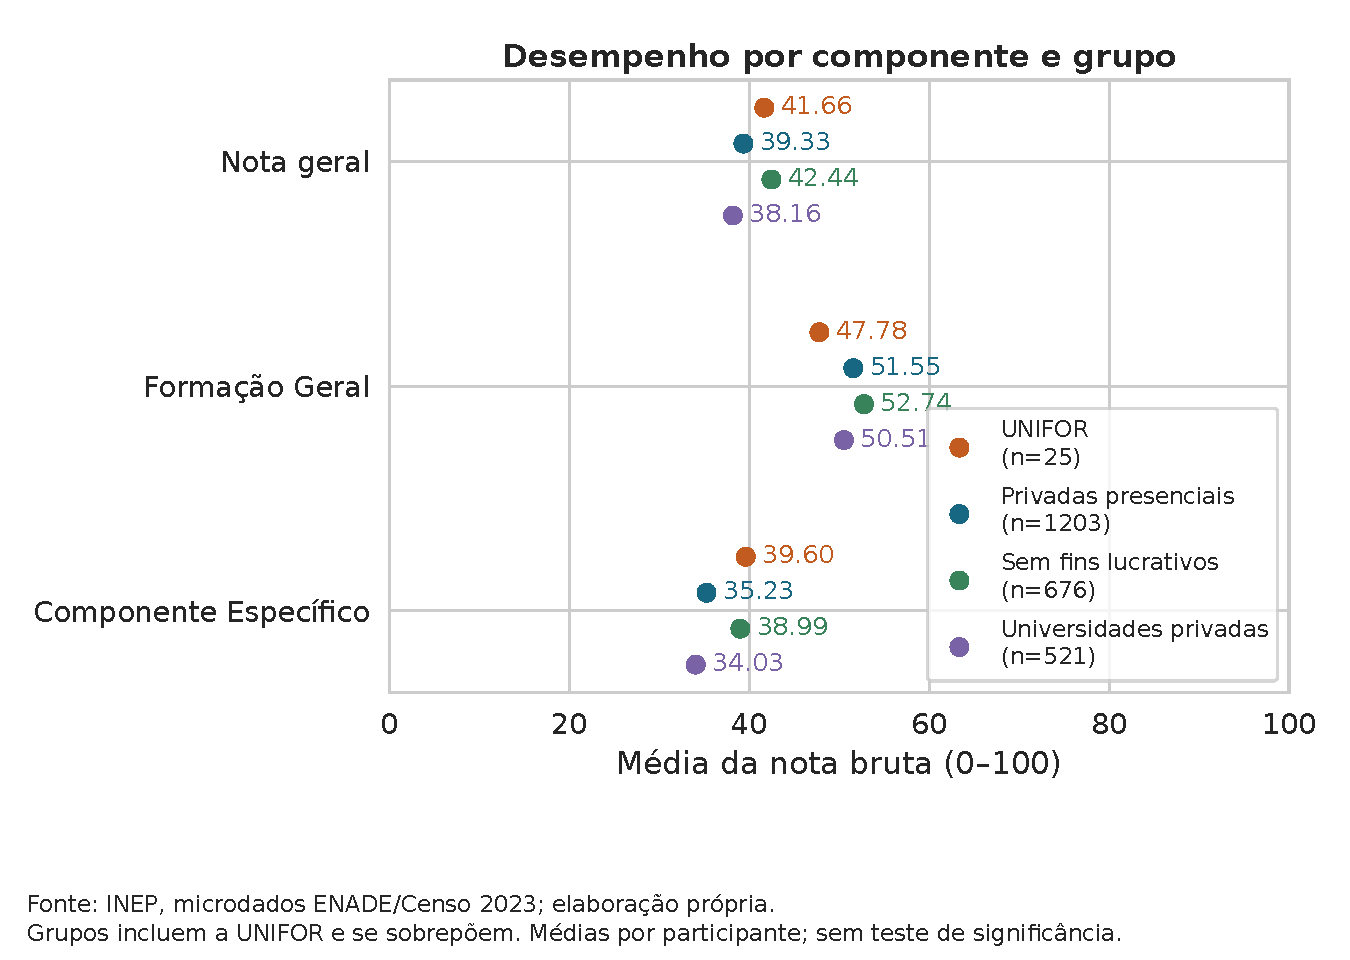
\includegraphics[width=\textwidth]{../resultados/graficos/comparacao_componentes_2023.pdf}
\caption{Médias por participante em grupos institucionais sobrepostos.}
\label{fig:medias}
\end{figure}
Na Figura~\ref{fig:medias}, a UNIFOR apresenta média geral e CE maiores que
o conjunto privado, mas FG menor. A média geral das instituições sem fins
lucrativos, \MediaSemFinsGeral{}, supera a da UNIFOR. Assim, a interpretação
depende do referencial institucional, sem sustentar um ranking de qualidade.

\begin{table}[H]
\centering\small
\caption{Notas publicadas: UNIFOR e demais privadas; escala 0--100.}
\label{tab:resumo}
\begin{tabular}{llrrrr}
\toprule
Grupo & Nota & n & Média & Mediana & DP \\
\midrule
UNIFOR & Geral & 25 & 41,66 & 41,20 & 9,30 \\
UNIFOR & FG & 25 & 47,78 & 50,60 & 12,37 \\
UNIFOR & CE & 25 & 39,60 & 38,00 & 10,72 \\
Demais privadas & Geral & 1178 & 39,28 & 38,45 & 12,03 \\
Demais privadas & FG & 1178 & 51,63 & 51,30 & 16,01 \\
Demais privadas & CE & 1178 & 35,14 & 33,80 & 13,54 \\
\bottomrule
\end{tabular}

\par\smallskip\footnotesize Fonte: INEP, ENADE/Censo 2023; elaboração própria.
DP: desvio-padrão amostral. As demais privadas excluem a UNIFOR.
\end{table}
Retirando a UNIFOR do referencial, suas diferenças de média são
\DiferencaGeral{} pontos na nota geral, \DiferencaFG{} na FG e
\DiferencaCE{} no CE. A Tabela~\ref{tab:resumo} mostra menor dispersão
na UNIFOR em FG e CE; seus 25 resultados, porém, limitam a estabilidade da descrição.

\clearpage
\section{Relação entre Formação Geral e Componente Específico}
\begin{figure}[H]
\centering
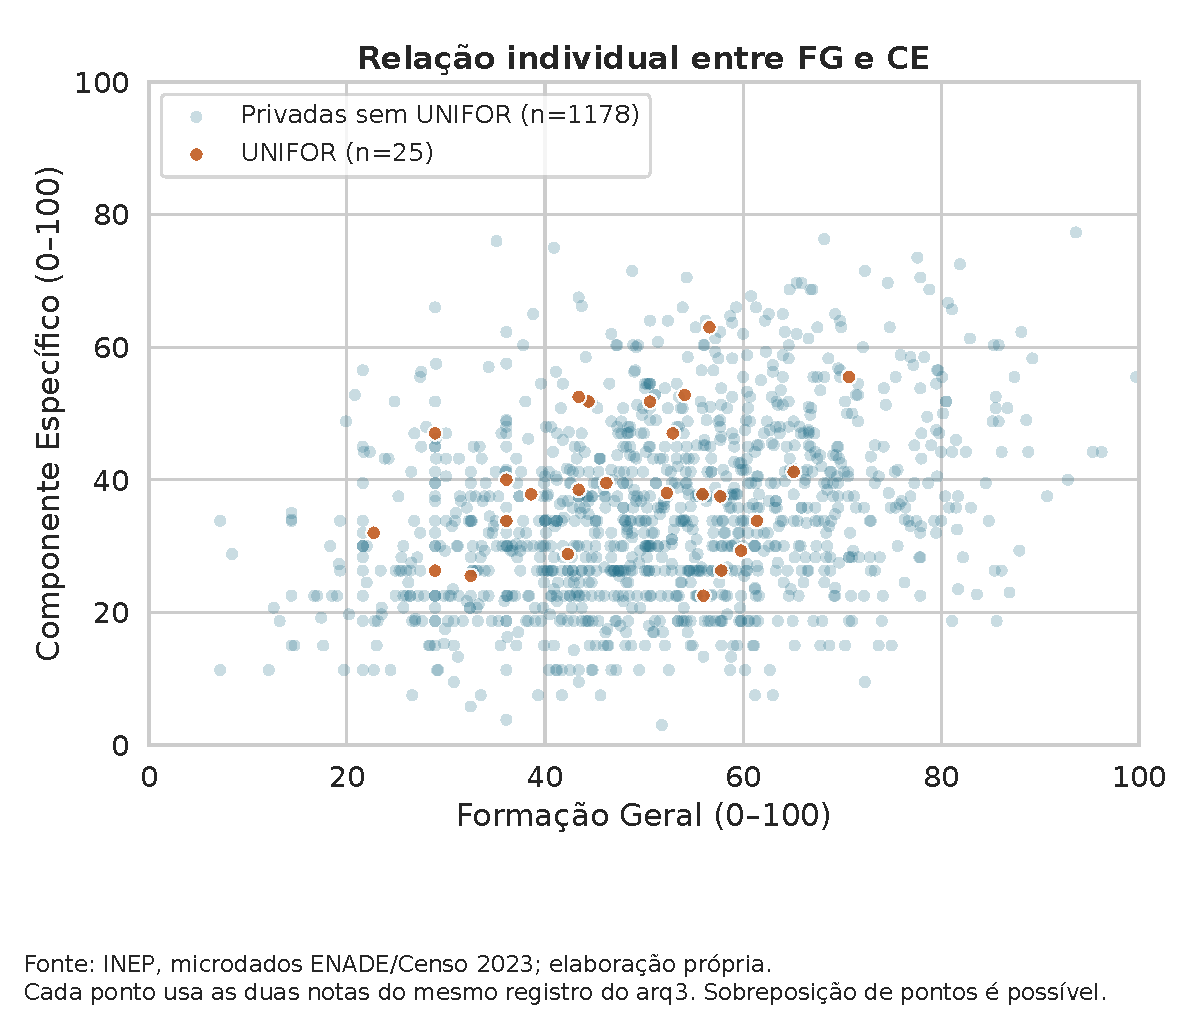
\includegraphics[width=.94\textwidth]{../resultados/graficos/relacao_fg_ce_2023.pdf}
\caption{Notas de FG e CE emparelhadas no próprio arq3.}
\label{fig:relacao}
\end{figure}
A Figura~\ref{fig:relacao} indica associação positiva entre as duas notas,
com ampla dispersão: FG maior não determina CE maior para cada estudante.
A correlação de Pearson é \CorrelacaoUnifor{} na UNIFOR e
\CorrelacaoDemais{} nas demais privadas, usando respectivamente 25 e
\NotasSemUnifor{} pares completos do mesmo arquivo. Não se correlacionam
registros de pessoas presumidas entre arquivos.

No universo privado completo, $r=\CorrelacaoPrivadas{}$, com
\TotalNotas{} pares. As estatísticas dos subconjuntos institucionais estão
nas tabelas complementares do notebook.
Os coeficientes resumem a amostra de notas publicadas; não foram feitos testes
de significância ou ajustes por perfil. O resultado da UNIFOR é especialmente
sensível ao tamanho reduzido da amostra. A diferença entre coeficientes não
constitui diferença estatisticamente comprovada entre instituições.

\clearpage
\section{Partes objetivas e discursivas}
\begin{figure}[H]
\centering
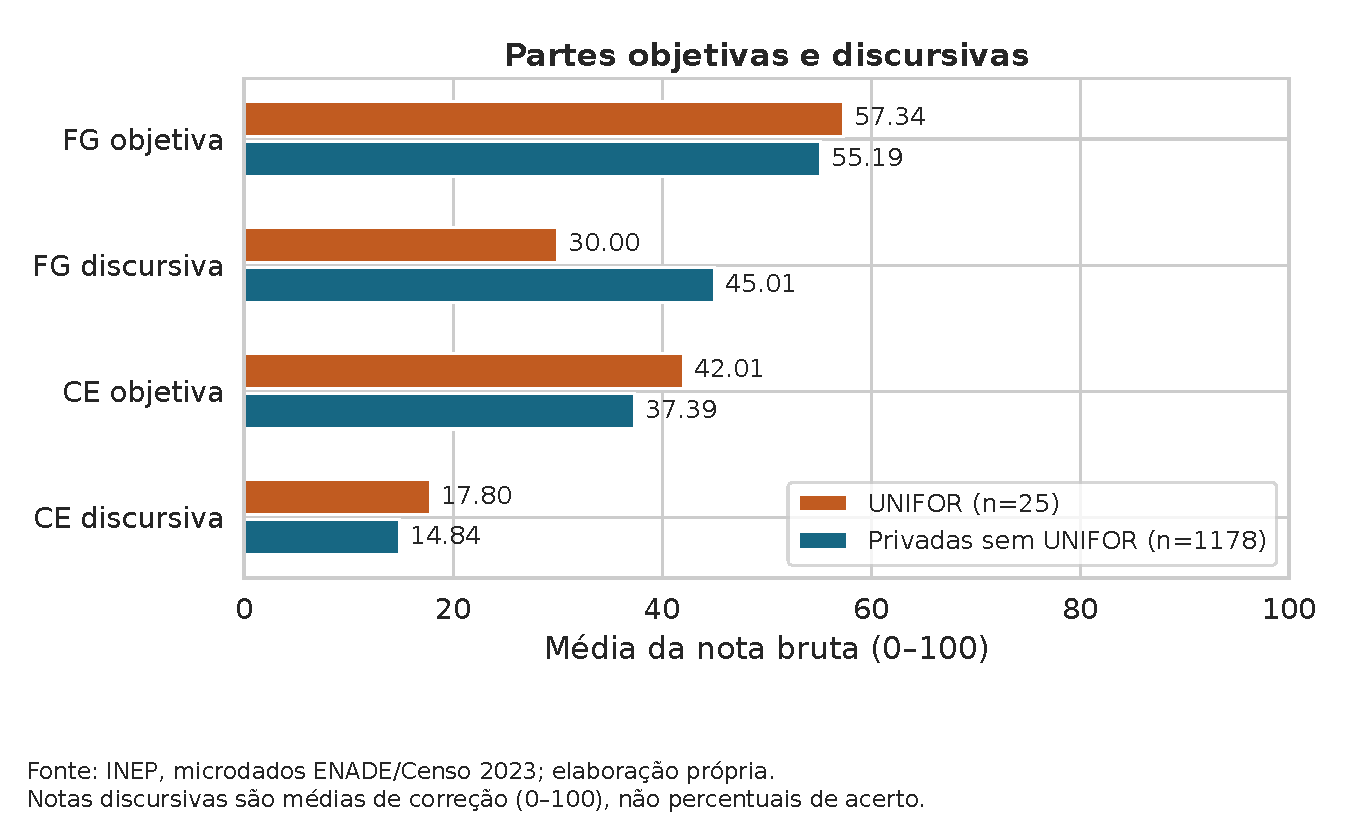
\includegraphics[width=\textwidth]{../resultados/graficos/partes_prova_2023.pdf}
\caption{Médias das partes da prova: 25 notas na UNIFOR e 1.178 nas demais privadas.}
\label{fig:partes}
\end{figure}
A Figura~\ref{fig:partes} localiza a principal fragilidade relativa da UNIFOR:
a FG discursiva tem média \MediaDiscursivaFGUnifor{}, contra
\MediaDiscursivaFGDemais{} nas demais privadas. A FG objetiva é maior,
\MediaObjetivaFGUnifor{} ante \MediaObjetivaFGDemais{}. Logo, a menor FG
total não decorre de menor média objetiva. No CE, ambas as partes têm médias
maiores na UNIFOR. As discursivas são notas de correção, não taxas de acerto.

\begin{table}[H]
\centering\small
\caption{Diferenças entre as médias das partes, em pontos (0--100).}
\begin{tabular}{lrrr}
\toprule
Parte & UNIFOR & Demais privadas & $\Delta$ (pontos) \\
\midrule
FG objetiva & 57,34 & 55,19 & 2,15 \\
FG discursiva & 30,00 & 45,01 & -15,01 \\
CE objetiva & 42,01 & 37,39 & 4,63 \\
CE discursiva & 17,80 & 14,84 & 2,96 \\
\bottomrule
\end{tabular}

\par\smallskip\footnotesize Fonte: INEP, ENADE/Censo 2023; elaboração própria.
$\Delta$: UNIFOR menos demais privadas.
\end{table}
A Nota Técnica nº 12/2024 define FG com pesos 65\% objetiva e 35\%
discursiva, CE com 90\% e 10\%, e nota geral com 25\% FG e 75\% CE
\cite{notaindividual}. Esses pesos reproduzem os dados dentro do arredondamento.
As descrições 60/40 e 85/15 do XLSX local são incompatíveis com as notas e não
foram utilizadas. Não se recalculam ou substituem as notas oficiais publicadas.

\clearpage
\section{Acertos nas questões de Formação Geral}
\begin{figure}[H]
\centering
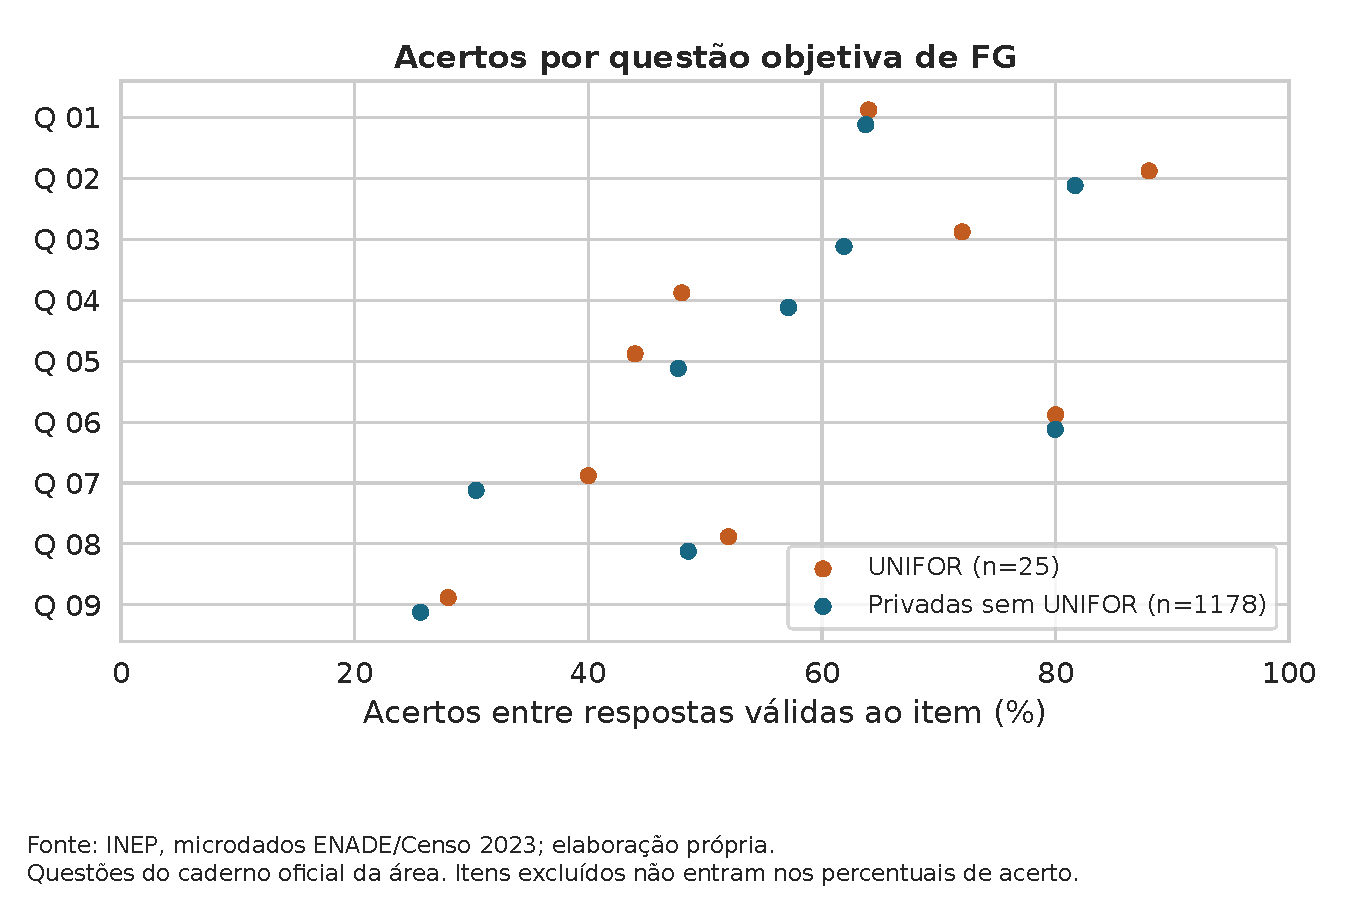
\includegraphics[width=\textwidth]{../resultados/graficos/itens_fg_2023.pdf}
\caption{Acertos nas nove questões objetivas de FG; nenhuma excluída no recorte.}
\label{fig:fg}
\end{figure}
A Figura~\ref{fig:fg} usa os vetores de acertos e o gabarito final do arq3,
conferidos com respostas do mesmo registro e com a sequência do gabarito oficial
\cite{gabarito}. O denominador de cada questão é 25 na UNIFOR e 1.178 nas
demais privadas. Branco ou marcação múltipla entram como erro quando assim
codificados oficialmente; itens excluídos não seriam tratados como erro.

Na questão 3, a UNIFOR tem 72,0\% de acertos (18/25), contra 61,9\%
(729/1.178), diferença de 10,1 pontos percentuais. Na questão 4, registra 48,0\%
(12/25), contra 57,1\% (673/1.178), diferença de $-9,1$ pontos percentuais.
As variações entre questões coexistem com a média objetiva maior da UNIFOR.

Uma resposta na UNIFOR altera o percentual em quatro pontos percentuais.
As diferenças por item são exploratórias, sem testes múltiplos ou diagnóstico
de competências. Os índices identificam questões do caderno de 2023; não
estabelecem equivalência com provas de outras áreas ou edições.

\clearpage
\section{Questões do Componente Específico}
\begin{figure}[H]
\centering
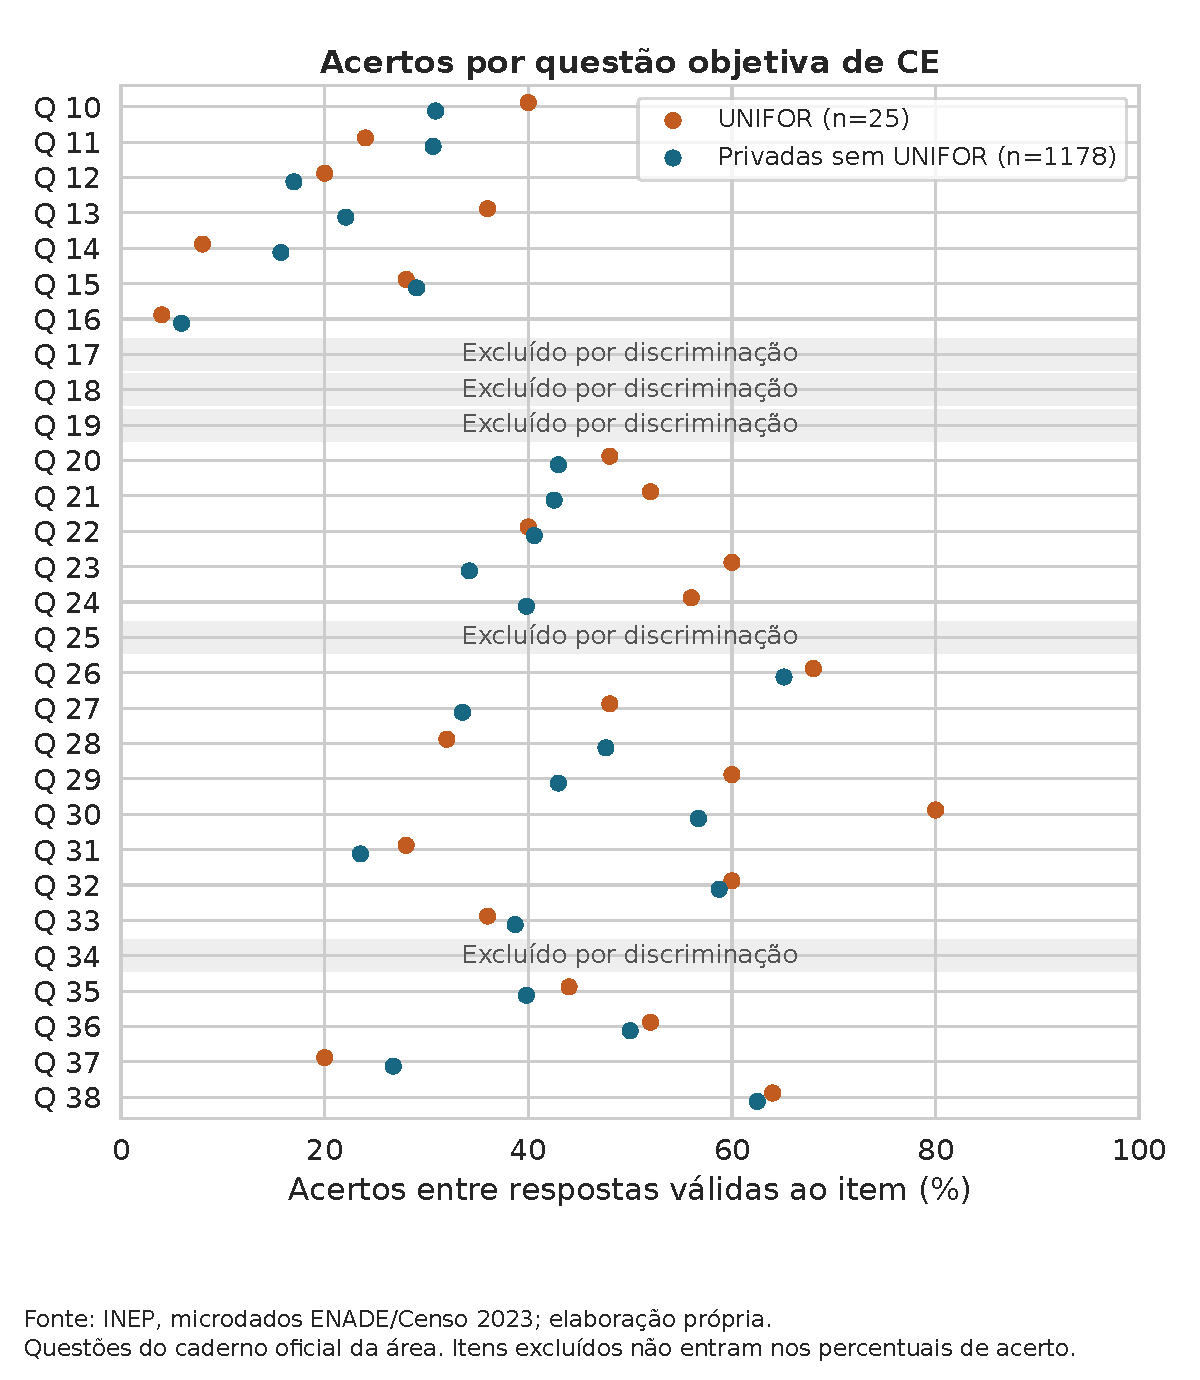
\includegraphics[width=\textwidth]{../resultados/graficos/itens_ce_2023.pdf}
\caption{Questões objetivas 10--38: 24 válidas e cinco excluídas por discriminação.}
\label{fig:ce}
\end{figure}
A Figura~\ref{fig:ce} exclui as questões 17, 18, 19, 25 e 34 do cálculo.
A UNIFOR tem 60,0\% na questão 23, ante 34,2\% nas demais privadas
($+25,8$ pontos percentuais); na questão 28, 32,0\% ante 47,6\%
($-15,6$). Cada item válido usa 25 e 1.178 respostas, respectivamente.
São diferenças descritivas, sensíveis aos poucos participantes da UNIFOR.

\clearpage
\section{Perfil socioeconômico complementar}
\begin{figure}[H]
\centering
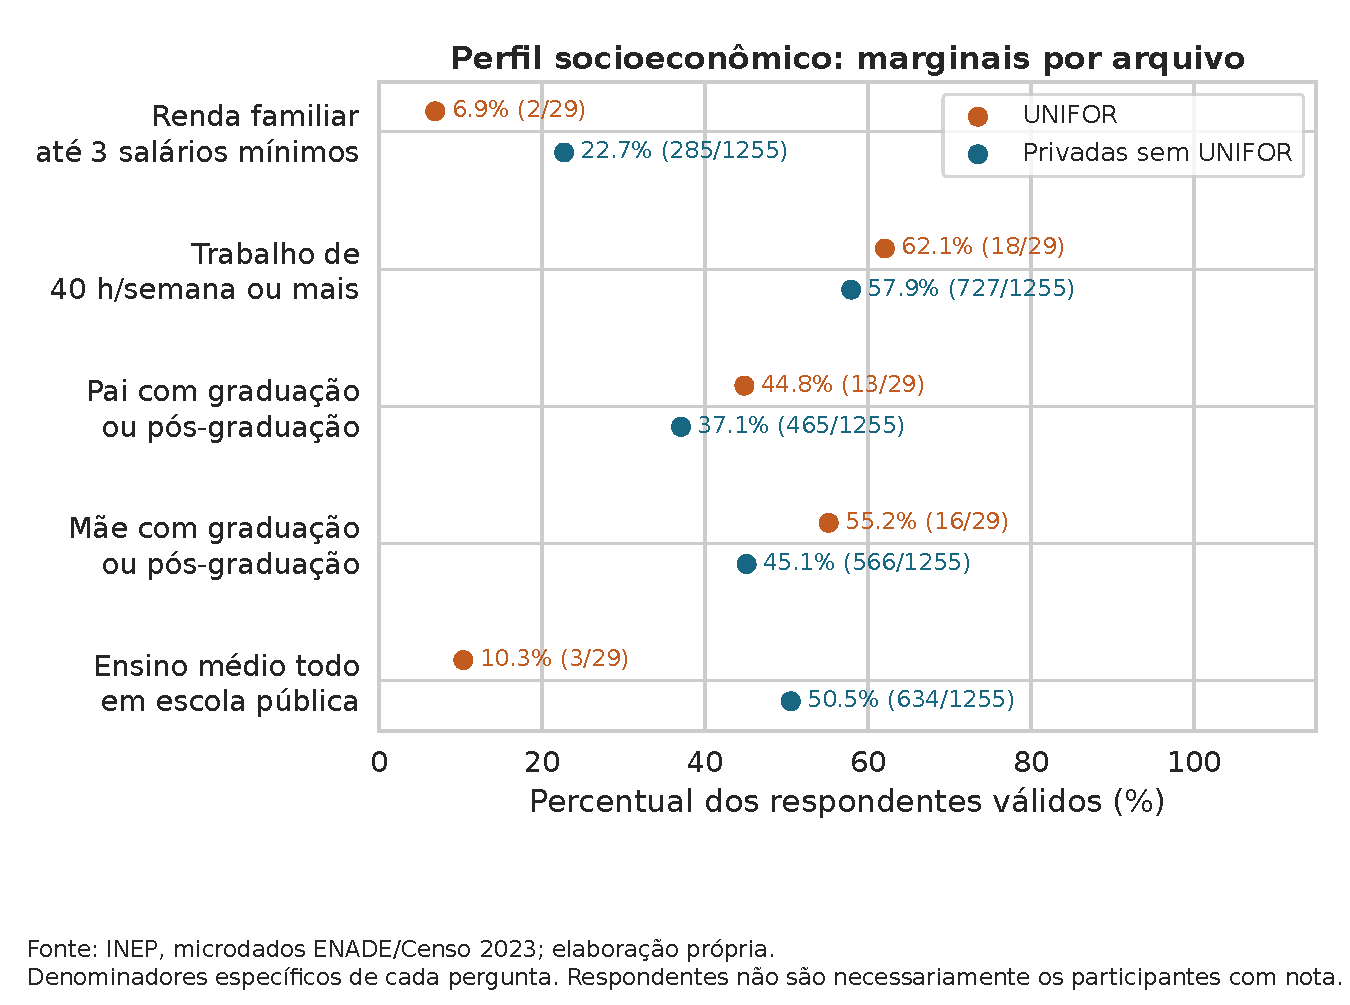
\includegraphics[width=\textwidth]{../resultados/graficos/perfil_socioeconomico_2023.pdf}
\caption{Proporções entre respondentes de cada pergunta, sem junções individuais.}
\label{fig:perfil}
\end{figure}
A Figura~\ref{fig:perfil} compara perfis marginais: ensino médio integralmente
público corresponde a \PerfilUniforEscola\% na UNIFOR (3/29), ante
\PerfilDemaisEscola\% nas demais privadas (634/1.255). Renda familiar até
três salários mínimos reúne \PerfilUniforRenda\% (2/29), ante
\PerfilDemaisRenda\% (285/1.255). São diferenças de composição relevantes
para contextualizar as médias, sem explicar causalmente os resultados.

Na UNIFOR, \PerfilUniforTrabalho\% trabalham 40 horas semanais ou mais;
\PerfilUniforPai\% têm pai com graduação ou pós-graduação e
\PerfilUniforMae\% têm mãe nessa condição. Nas demais privadas, os valores
são \PerfilDemaisTrabalho\%, \PerfilDemaisPai\% e \PerfilDemaisMae\%,
respectivamente. Trabalho exclui estágio e bolsas; as faixas de renda seguem
o questionário de 2023 \cite{questionario}.

Cada um dos cinco arquivos tem 29 respostas publicadas e uma ausência na
UNIFOR; nas demais privadas, 1.255 respostas e 133 ausências. Calculam-se os
percentuais sobre respostas válidas, não sobre inscritos ou notas.
Denominadores iguais entre arquivos não provam identidade dos respondentes.
As 29 respostas não podem ser relacionadas individualmente às 25 notas.

\clearpage
\section{Discussão, limitações e conclusão}
O aprofundamento distingue três resultados: a média geral da UNIFOR supera a
do conjunto privado; o CE contribui para essa diferença; a FG discursiva é
o principal ponto de atenção relativo. Isso sugere examinar pedagogicamente
esse componente, sem atribuir seu resultado a currículo, renda, trabalho ou
qualquer mecanismo que os dados não permitem identificar.

As médias gerais também variam com a ponderação: no universo privado,
\MediaPrivadasGeral{} por participante e \MediaCursosGeral{} com peso igual
por curso. Dos \TotalCursos{} cursos, \CursosComNotas{} têm notas publicadas;
\CursosDestaque{} têm ao menos dez. Cursos sem notas não recebem média zero.
As tabelas completas e os diagramas de distribuição permanecem no notebook.

O perfil socioeconômico da UNIFOR difere do referencial. Entretanto, não é
possível ajustar as notas por características individuais em arquivos distintos.
As correlações entre proporções socioeconômicas e médias, disponíveis no
notebook para 47 cursos com ao menos dez notas e dez respostas, têm unidade
curso e peso igual. Não demonstram efeitos sobre estudantes: usar resultados
agregados para inferir relações individuais incorreria em falácia ecológica.

O sigilo exclui notas de cursos com apenas uma presença válida e respostas
de cursos com apenas um respondente \cite[pp.~7--8]{manual}. Não se recuperam
esses valores. Ausência na prova, não resposta, supressão e pequenas amostras
limitam a representatividade. A correlação FG--CE é descritiva e não substitui
análise dos componentes ou inferência com pressupostos explícitos.

O curso ENADE 1125254, IES 137, permanece no universo apesar de não ter vínculo
com o cadastro de cursos do Censo; sua IES foi localizada. Não há substituição
por código semelhante. A categoria ENADE 8 dessa IES é compatível com o
indicador confessional, embora o indicador comunitária seja zero. Esses casos
são preservados e documentados, sem alterar o recorte para obter contagens esperadas.

Não há microdados locais de ENADE ou Censo 2021; a comparação com Ciência da
Computação da UNIFOR permanece pendente. Mesmo com esses arquivos, notas brutas
de áreas e anos diferentes não mediriam diretamente superioridade entre cursos.

Conclui-se que a avaliação por componentes e questões acrescenta informação
à média geral: o desempenho relativo positivo em CE convive com menor nota
discursiva de FG. O resultado oferece um diagnóstico descritivo da amostra
publicada, sem demonstrar qualidade global ou superioridade estatística do curso.

\clearpage
\begin{thebibliography}{9}
\bibitem{enade} INEP. \textit{Microdados do ENADE 2023}. Brasília: Inep.
Dados oficiais e dicionário XLSX do ZIP local (versão de abril de 2025).
\href{https://www.gov.br/inep/pt-br/acesso-a-informacao/dados-abertos/microdados/enade}{Portal de microdados ENADE}.

\bibitem{censo} INEP. \textit{Microdados do Censo da Educação Superior 2023}.
Cadastros de cursos e instituições e dicionário oficiais do ZIP local.
\href{https://www.gov.br/inep/pt-br/acesso-a-informacao/dados-abertos/microdados/censo-da-educacao-superior}{Portal de microdados do Censo Superior}.

\bibitem{manual} INEP. \textit{Manual do usuário -- Microdados do Enade 2023}.
Atualizado em 11 abr. 2025. Documento integrante do ZIP oficial, especialmente
pp.~6--11. Consultado localmente em 18 out. 2026.

\bibitem{questionario} INEP. \textit{Questionário do Estudante Enade 2023}.
Documento integrante do ZIP oficial. Questões 4, 5, 8, 10 e 17.
Consultado localmente em 18 out. 2026.

\bibitem{notaindividual} INEP. \textit{Nota Técnica nº 12/2024/CEI/CGGI/DAES-INEP}.
Cálculo da nota final do estudante no Enade 2023 e correlação ponto-bisserial,
seção 4.
\href{https://download.inep.gov.br/educacao_superior/enade/notas_tecnicas/2024/nota_tecnica_12_calculo_nota_final_enade_2023.pdf}{Documento oficial}.
Consulta em 18 out. 2026.

\bibitem{gabarito} INEP. \textit{Enade 2023: Engenharia da Computação --
gabarito definitivo}. Questões objetivas 1--38.
\href{https://download.inep.gov.br/enade/provas_e_gabaritos/2023_GB_engenharia_da_computacao.pdf}{Gabarito oficial}.
Consulta em 18 out. 2026. Exclusões estatísticas posteriores seguem o arq3.

\bibitem{conceito} INEP. \textit{Nota Técnica nº 6/2024: metodologia de
cálculo do Conceito Enade 2023}.
\href{https://download.inep.gov.br/educacao_superior/enade/notas_tecnicas/2024/nota_tecnica_6_metodologia_calculo_conceito_enade_2023.pdf}{Documento oficial}.
\end{thebibliography}
\end{document}
